% !TEX root = ../../buch.tex
% problemstellung.tex -- Beispiel-File für die Beschreibung des Problems
%
% (c) 2020 Prof Dr Andreas Müller, Hochschule Rapperswil
%
\section{Problemstellung
\label{burgers:section:problemstellung}}
\rhead{Problemstellung}

	Das Ziel dieses Papers ist die numerische Berechnung der Lösung für die Gleichung von Burgers mit ihren Schwierigkeiten aufzuzeigen.



	\subsection{Numerische Wettervorhersage}
	\label{burgers:sec:nwp}

	Der numerische L\"osungsansatz von nichtlinearen partiellen Differentialgleichungen entpuppte sich bereits in den 30er Jahren als eine grosse Herausforderung.
	Lewis Fry Richardson (1881 -- 1953) war ein britischer Mathematiker und Physiker, welcher als einer der Ersten versuchte, das Wetter mittels numerischer Lösung der fundamentalen Differentialgleichungen zu prognostizieren.
	F\"ur eine Vorhersage von sechs Stunden ben\"otigte er mit seinem Team gegen sechs Wochen.
	Das Resultat war ern\"uchternd beziehungsweise schlichtweg falsch.
	Es stellte sich heraus, dass Richardson einen Algorithmus verwendete welcher numerisch instabil war.
	Im Verlauf des Papers wird aufgezeigt, welcher Fehler dabei begangen wurde.

	\subsection{Notation}

     \begin{figure}
       \centering
       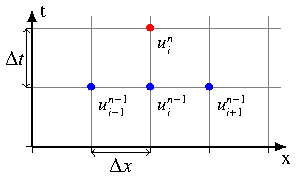
\includegraphics[width=.8\textwidth]{papers/burgers/BurgersEquation/tikz/Gitter/gitter.pdf}
       \caption{Notation Diskretisierung}
       \label{burgers:fig:Disk}
     \end{figure}


     Wie es bei der numerischen L\"osung von partiellen Differentialgleichungen \"ublich ist, wird die Raum-Zeit-Ebene  diskretisiert.
     Die gew\"ahlte Notation f\"ur die Diskretisierung kann \autoref{burgers:fig:Disk} entnommen werden, wobei $u_i^n$ der zu berechnende Punkt ist.
     Weiter ist $i-1$ Schritt zur\"uck im Raum und $n-1$ ein Schritt zur\"uck in der Zeit.
     $\Delta x$ und $\Delta t$ sind die Schrittgr\"ossen in der entsprechenden Dimension, welche entgegengesetzt \autoref{burgers:fig:Disk} nicht gleich gross sein m\"ussen.
